% 本文是机械臂设计章节中的机构选型章节
% 作者:谭正
% 上次更新:20点45分2020年1月12日

\subsection{机构选型}

机械臂部分的机构主要是传动机构,其选择的基本原则是满足强度要求的前提下选取最小质量的传动件。
本小节将一一介绍本机械臂传动机构选择的过程。

\subsubsection{减速机构选型}

正如小节\ref{subsec:roughCal}所述,云台处需要在加速时(启动或停下)提供超大的扭矩。
其中,为了减小停止运动时,由整个机械臂带来的巨大的惯性力对电机的危害,我们在设计传动机构时选择了单向自锁的蜗轮蜗杆传动。

在第一次设计时,选取了如图~\ref{fig:RP_trans}所示的蜗轮蜗杆外加行星轮减速的两级减速机构设计。
该机构减速比约为100左右,其中蜗轮蜗杆减速比达到了15。

\begin{figure}[!h]
    \centering
    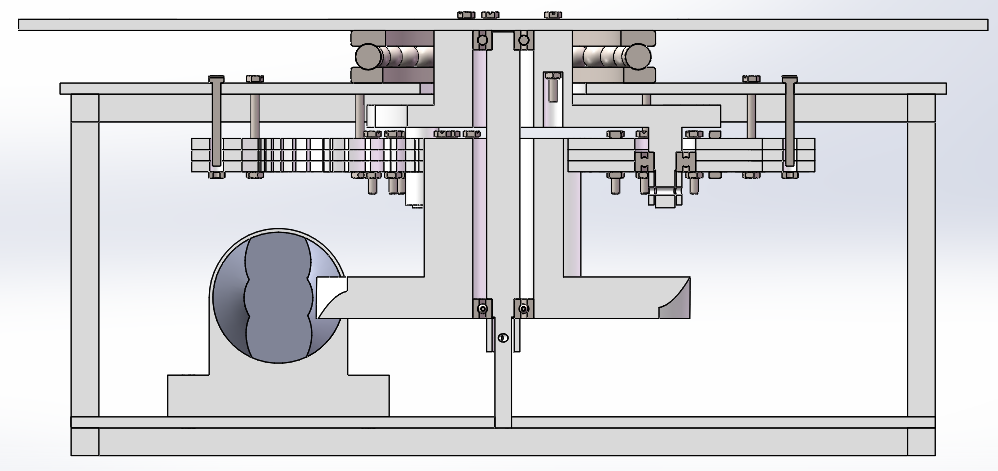
\includegraphics[width=\textwidth]{RP_transmission_design.png}
    \bicaption[云台减速机构设计(第一次)]{云台减速机构设计(第一次)}{Transmission design of rotational platform (original design)}
    \label{fig:RP_trans}
\end{figure}

但考虑到过大的减速比会使平台的转速过慢,而且多级传动时,为保证精度,一般将传动比高的减速机构布置在低速级\cite{MMDM}。因此再后来的改进设计中,我们更换了方案,只采用一对蜗轮蜗杆副传动。

首先在淘宝上找到一家销售蜗轮蜗杆副的店家,得到他们的尺寸如图~\ref{fig:worm_shaft}所示。

\begin{figure}[!h]
    \centering
    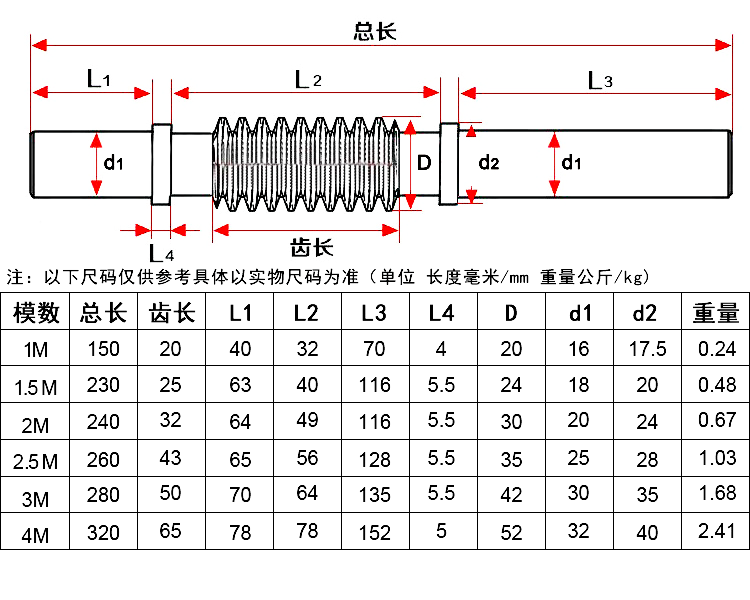
\includegraphics[width=0.8\textwidth]{worm_shaft.png}
    \bicaption[淘宝蜗杆尺寸图]{蜗杆尺寸图}{Worm size chart}
    \label{fig:worm_shaft}
\end{figure}

查阅相关资料得到蜗轮蜗杆副的设计如式~\ref{eq:worm_gear_design}。

\begin{equation}
    \label{eq:worm_gear_design}
    m^2d_1 \geq (\frac{15000}{\sigma_{HP}z_2})^2KT_2
\end{equation}

取蜗轮蜗杆传动中的机械效率$\eta = 0.7$可得到依据输入扭矩$T_1$的设计式~\ref{eq:worm_design}。

\begin{equation}
    \label{eq:worm_design}
    m^2d_1\geq(\frac{15000}{\sigma_{HP}z_2})^2K(0.7iT_1),i=\frac{z_2}{z_1}
\end{equation}

淘宝上所购的的蜗杆都是单头蜗杆,故有$m^2d_1 \geq f(i)$;所购的的蜗杆和蜗轮都是45号钢的材质,查表得到其许用接触应力$\sigma_{HP} = 475 Mpa$。
故作$f(i)$图像如图~\ref{fig:icurve}所示。

\begin{figure}
    \centering
    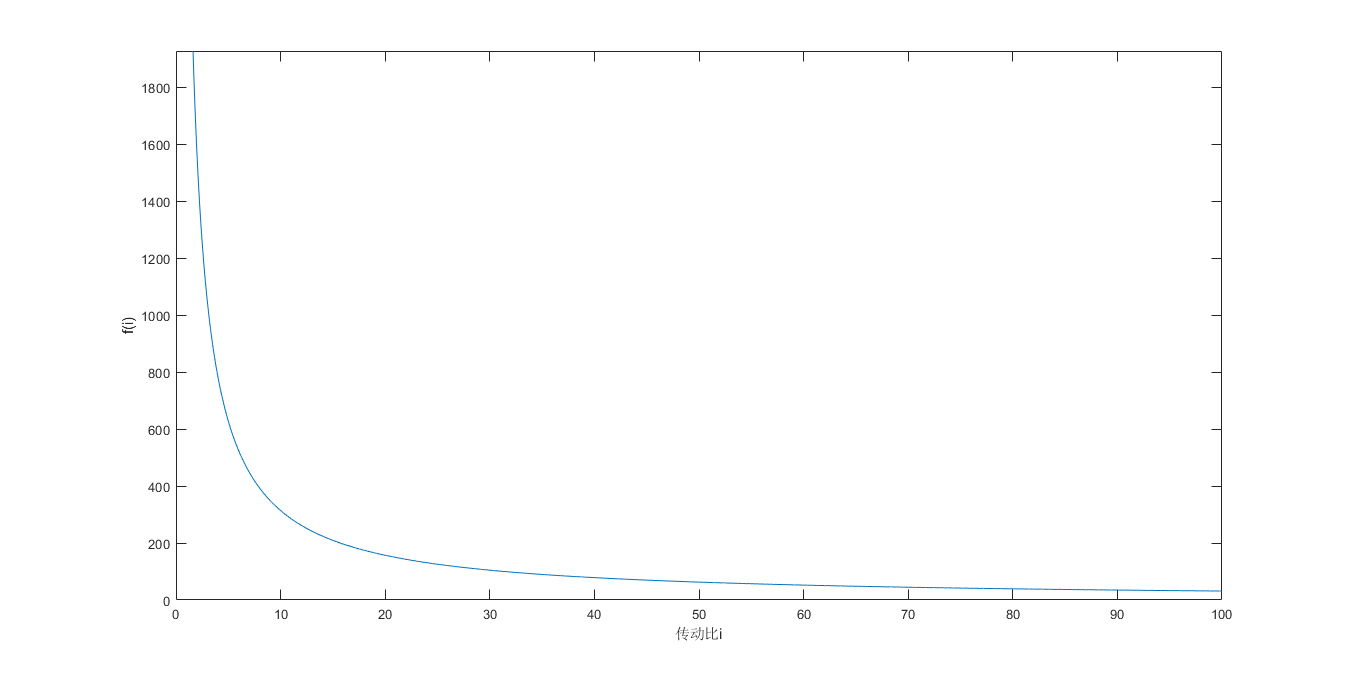
\includegraphics[width=0.8\textwidth]{icurve.png}
    \bicaption[蜗杆尺寸和传动比的关系]{f(i)的函数图像}{Function image of f (i)}
    \label{fig:icurve}
\end{figure}

由于这里已经选取了最大额定负载为$4.5 N\cdot M$的电机,所以为了使输出扭矩满足要求,该处传动比选择为$i = 55$,带入计算得到$m_2d_1\geq f(i) = 60.17 mm^3$。
故选取淘宝上模数为$2$的蜗杆,再带入验算式~\ref{eq:worm_check}。计算得到$\sigma_H = 492 MPa \geq [\sigma_{HP}]$。故不合乎要求,应选取更大的蜗杆。重新选取淘宝上模数为$2.5$的蜗杆,带入验算式~\ref{eq:worm_check}得到$\sigma_H = 367 MPa \leq [\sigma_{HP}]$,合乎强度要求。

\begin{equation}
    \label{eq:worm_check}
    \sigma_H = Z_E \sqrt{\frac{9400 T_2}{d_1 d_2^2}K_A K_V K_\beta} \leq \sigma_{HP}
\end{equation}

同样的道理,由于大臂的传动需要输出的扭矩约为$100 N \cdot M$,参照上述选取规则,选用3模30齿的蜗轮蜗杆副进行传动。

而因为在臂上不是很方便自己布置开式减速机构,故另外两个关节依靠淘宝上十分容易购买的直接和电机相连的减速箱来进行减速。这样虽然转速很慢,但扭矩能够保证,我们也是进行了一番取舍才选择了这种方案。

\subsubsection{传动机构选型}

对于布置在机械臂上的电机,其越接近根结点(图~\ref{fig:robot_motion}中A结点),越有利于减轻各个关节处的负载,故在实际布置时,我们往往使电机距离铰接处较远,这时需要机构把电机输出的运动往结点传递。本小节讨论的机构即是进行这类运动传输的机构。

由于中心距较大,我们首先排除了使用齿轮的方案。考虑到传送的扭矩比较大,不能使用普通带传动。而链传动的重量也不小,而且传动不平稳,在这种场合布置还可能有较大垂度,故我们最后选取了实惠又高效的同步带传动。并选取最大的尺寸以尽量减少同步带工作时的紧边拉力。